\subsection{Creep of a thick-walled cylinder}
\label{subsec:Mc1}

\subsubsection{Definition}
\label{subsubsec:Mc1_def}

In this example, creep behavior of a thick-walled cylinder is discussed, which is subjected to a constant inner normal pressure.

\subsubsection{Solution}
\label{subsubsec:Mc1_sol}

The inner and the outer radius of the cylinder are $4\,$mm and $6.4\,$mm respectively, at a height of $1\,$mm. Quadrilateral elements are used for the spatial discretization of the axisymmetric finite element model (cf. Fig.~\ref{Mc_fig:meshcrp}). The boundary conditions are as follows: normal pressure $p=2.515\,$MPa at the inner surface and zero normal stress at the outer surface. Furthermore, displacements in axial direction are suppresed at the top and the bottom surfaces. 
%
\begin{figure}[!htb]
\centering
\includegraphics[scale=0.3]{PART_II/M/mesh_crp}
\caption{Finite element grid of the thick-walled cylinder}
\label{Mc_fig:meshcrp}
\end{figure}

A homogeneous initial stress distribution is assumed in the domain, applying the following values for the coefficients of the stress tensor in cylindrical coordinates: $\sigma_{rr}^0=\sigma_{\theta\theta}^0=\sigma_{zz}^0=-50\,$Pa. The parameters of Norton's creep model are given in Table~\ref{Mc_tab:creep_norton}.

\begin{table}[!htb]
\centering
\caption{Material parameters of Norton's creep model}
\label{Mc_tab:creep_norton}
\begin{tabular}{llll}
\toprule
Symbol & Parameter & Value & Unit \\
\midrule
$E$      & Young's modulus       & $137.8$                & GPa \\
$\nu$    & Poisson's ratio       & $0.48$                 & -- \\
$\alpha$ & Norton model factor   & $6.415\times 10^{-10}$ & -- \\
$n$      & Norton Model exponent & $4$                    & -- \\
\bottomrule
\end{tabular}
\end{table}

The numerical results can be compared with Balley's analytical solution for the rate of radial displacements
%
\[
  \dot u_{r} =\alpha \dfrac{3^{\frac{n+1}{2}}}{2n^n}\dfrac{r_{a}^2\;r_{b}^2\;p^n}{(r_{b}^{2/n}-r_{a}^{2/n})r}
%% \label{Mc_eq:balleyu}
\]
and for the equilibrated state of the first stress invariant
\[
  \sigma_v =\dfrac{2\sqrt 3}{2n} \dfrac{p\;\left(r_b/r\right)^{\frac{2}{n}}}{(r_{b}/r_a)^{2/n}-1}
%% \label{Mc_eq:balleys}
\]

\subsubsection{Results}
\label{subsubsec:Mc1_res}

Figs.~\ref{Mc_fig:ex2_q} and \ref{Mc_fig:ex2_ur} show the distribution of the first stress invariant $\sigma_v$ and of radial displacements along the cross section of the sample wall compared to the pure elastic solution. This demonstrates that $\sigma_v$ decreases at about $26\,$\% at the inner surface of the thick-walled cylinder until the asymptotic creep state is reached. In contrast, the radial displacements increase at about $200\,$\%.

\begin{figure}[H]
\centering
\includegraphics[scale=0.4]{PART_II/M/ex2_q}
\vspace{-3mm}
\caption{Profiles of the first stress invariant during creep at different times, $t=5,\,25,\,50\,$sec compared to the elastic solution}
\label{Mc_fig:ex2_q}
\end{figure}

\begin{figure}[H]
\centering
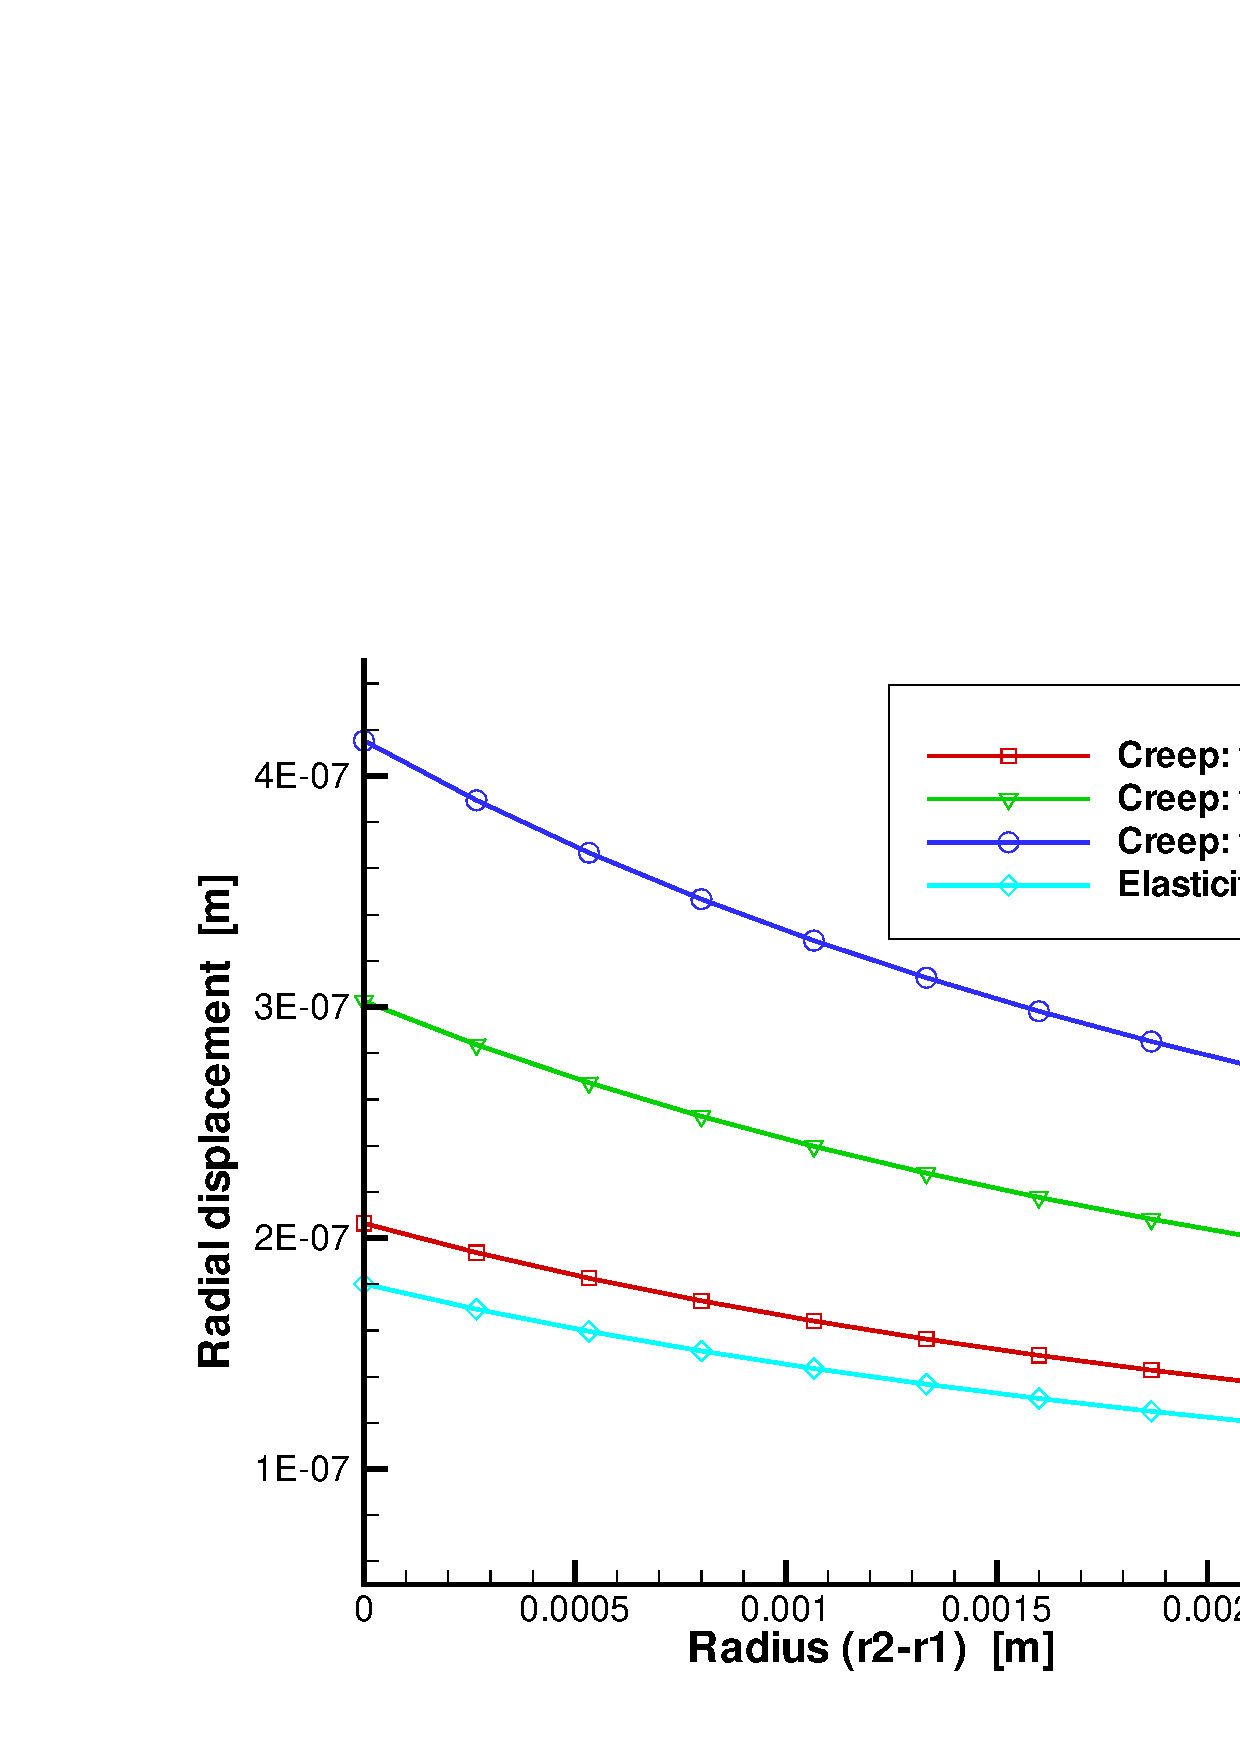
\includegraphics[scale=0.4]{PART_II/M/ex2_ur}
\vspace{-3mm}
\caption{Profiles of radial displacements during creep at different times, $t=5,\,25,\,50\,$sec compared to the elastic solution}
\label{Mc_fig:ex2_ur}
\end{figure}
